\documentclass{beamer}
\usetheme{Madrid}

\usepackage{amsmath, amssymb, amsthm}
\usepackage{graphicx}
\usepackage{listings}
\usepackage{gensymb}
\usepackage[utf8]{inputenc}
\usepackage{hyperref}
\usepackage{gvv}

\begin{document}

\title{ANALOG ASSIGNMENT}
\author{EE23BTECH11016 - Dure Aditi Rajesh$^{*}$}
\date{}
\frame{\titlepage}

\begin{frame}
\frametitle{Question}
\begin{enumerate}
\item The peak voltage of an AC supply is 300 V. What is the rms voltage?
\item The rms value of current in an AC circuit is 10 A. What is the peak current?
\end{enumerate} \hfill(NCERT)
\end{frame}

\begin{frame}{allowframebreaks}
\frametitle{Solution: Theory}
\begin{table}[!h]

  \centering
  \begin{tabular}{|c|c|c|}
    \hline
    parameter & value & description \\
    \hline
    $V(t)$ & $V_{\text{0}} \cdot \sin(2\pi ft + \phi)$ & voltage in terms of time \\
    \hline
    $I(t)$ & $I_{\text{0}} \cdot \sin(2\pi ft + \phi)$ & current in terms of time \\
    \hline
    $V_0$ & $300 \, \text{V}$ & peak voltage \\
    \hline
    $V_ \text{rms}$ & $\sqrt{\frac{1}{T} \int_{0}^{T} [V(t)]^2 \, dt}$ & rms value of Voltage \\
    \hline 
    $I_ \text{rms}$ & $10 \, \text{A}$ & rms value of current\\
    \hline
    $I_0$ & $\sqrt{2} \times I_{\text{rms}}$ & peak current \\
    \hline
    $f$ & $50 \, \text{Hz}$ & frequence of the sinosoidal wave. \\
    \hline
    $T$ & $0.02 \, \text{s}$ & time period of sinosoidal wave. \\
    \hline
  \end{tabular}


\caption{Input Parameter Table}
\label{tab:input_parameters}
\end{table}
\end{frame}
\begin{frame}
\frametitle{Theory}

\begin{align}
V_{\text{rms}}^2 &= {\frac{1}{T} \int_{0}^{T} [V(t)]^2 \, dt} \\
&= {f \int_{0}^{\frac{1}{f}} V_{\text{0}}^2 \cdot \sin^2(2\pi ft + \phi) \, dt} \\
&= \frac{1}{2} V_{0}^2 \left(1 - \frac{1}{f}\int_{0}^{\frac{1}{f}} \cos(4\pi ft + 2\phi) \, dt \right) \\
&= \frac{1}{2} V_{0}^2 \left(1 - \frac{1}{f}\left[\frac{\sin(4\pi ft + 2\phi)}{4\pi f}\right]_{0}^{\frac{1}{f}}\right) \\
&= \frac{1}{2} V_{0}^2 \left(1 - \frac{1}{f} \cdot \frac{\sin\left(4\pi + 2\phi\right) - \sin(0 + 2\phi)}{4\pi f}\right) \\
V_{\text{rms}} &= \frac{V_{0}}{\sqrt{2}} \label{eq:12.7.2_voltage}
\end{align}

\end{frame}
\begin{frame}
\frametitle{Theory}
To find the RMS voltage (\(V_{\text{rms}})\) when the peak voltage (\(V_{\text{0}})\) is 300V, you can use equation  \eqref{eq:12.7.2_voltage}

\begin{align}
V_{\text{rms}} &= \frac{300V}{\sqrt{2}} \approx 212.13V
\end{align}

\end{frame}
\begin{frame}
\frametitle{Theory}
 
\begin{align}
I_{\text{rms}}^2 &= {\frac{1}{T} \int_{0}^{T} [I(t)]^2 \, dt} \\
&= {f \int_{0}^{\frac{1}{f}} I_{\text{0}}^2 \cdot \sin^2(2\pi ft + \phi) \, dt} \\
&= \frac{1}{2} I_{0}^2 \left(1 - \frac{1}{f}\left[\frac{\sin(4\pi ft + 2\phi)}{4\pi f}\right]_{0}^{\frac{1}{f}}\right) \\
&= \frac{1}{2} I_{0}^2 \left(1 - \frac{1}{f} \cdot \frac{\sin\left(4\pi + 2\phi\right) - \sin(0 + 2\phi)}{4\pi f}\right) \\
I_{\text{rms}} &= \frac{I_{0}}{\sqrt{2}} \label{eq:12.7.2_current}
\end{align}
\end{frame}
\begin{frame}
\frametitle{Theory}
To find the peak current (\(I_{\text{0}}\)) when the RMS current (\(I_{\text{rms}}\)) is given, you can use equation  \eqref{eq:12.7.2_current}

\begin{align}
I_{\text{0}} \approx 10 \, \text{A} \times 1.414 \approx 14.14 \, \text{A}  
\end{align}
\end{frame}
\begin{frame}
\frametitle{Theory}
\begin{figure}[H]
    \centering
    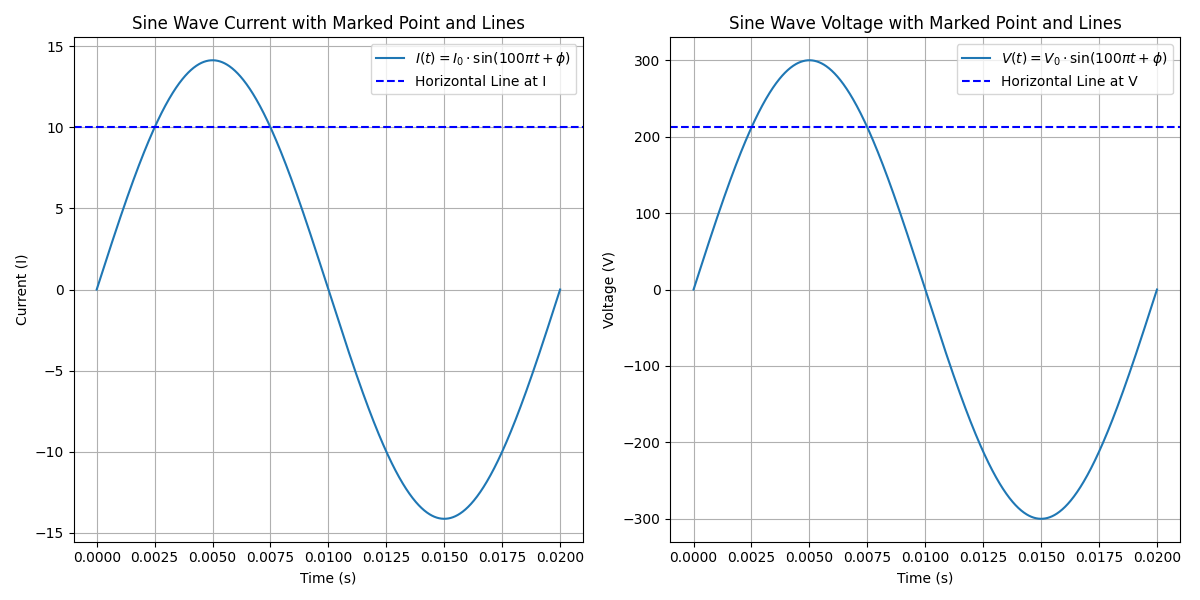
\includegraphics[scale = 0.5]{./figs/merged_sine_wave_plots.png}
\end{figure}
\end{frame}
\end{document}
